
\section{Own implementation: lid-driven cavity}

In my own implementation I implemented lid-driven cavity in 3D with D3Q19 model. The result of the simulation you can see on the Figure 10.

To compute streaming step and collision step I saved all $c_i$ and $t_p$ in the arrays:

\begin{lstlisting}
static const int LATTICEVELOCITIES[19][3] = {
    {0,-1,-1}, {-1,0,-1}, {0,0,-1}, {1,0,-1}, {0,1,-1},
    {-1,-1,0}, {0,-1,0}, {1,-1,0}, {-1,0,0}, {0,0,0},
    {1,0,0}, {-1,1,0}, {0,1,0}, {1,1,0}, {0,-1,1},
    {-1,0,1}, {0,0,1}, {1,0,1}, {0,1,1} };
static const double LATTICEWEIGHTS[19] = {
    1.0/36, 1.0/36, 2.0/36, 1.0/36, 1.0/36,
    1.0/36, 2.0/36, 1.0/36, 2.0/36, 12.0/36,
    2.0/36, 1.0/36, 2.0/36, 1.0/36, 1.0/36,
    1.0/36, 2.0/36, 1.0/36, 1.0/36 };
\end{lstlisting}

The main for loop looks like this:
\begin{lstlisting}
for(t = 0; t<=timesteps; t++){
    doStreaming( collide_field, stream_field,
        flag_field, xlength );
    swapFields(collide_field, stream_field);
    doCollision(collide_field, flag_field, &tau, xlength);
    treatBoundary( collide_field, flag_field,
        velocity_wall, xlength );
}
\end{lstlisting}

Function for streaming step is straightforward:
\begin{lstlisting}
void doStreaming(double *collideField, double *streamField,
int *flagField,int xlength){
  int x = 0, y = 0, z = 0;
  int i = 0;
  /* len is used to set values in lexicographic order
  "[ Q * ( z*len*len + y*len + x) + i ]" */
  int len = xlength + 2;
  /* sum of coordinates and velocity(X + Ci) */
  int sum[3];

  for(z=1; z<=xlength; z++) {
  for(y=1; y<=xlength; y++) {
  for(x=1; x<=xlength; x++) {
  for(i=0; i<Q; i++) {
    sum[0] = x - LATTICEVELOCITIES[i][0];
    sum[1] = y - LATTICEVELOCITIES[i][1];
    sum[2] = z - LATTICEVELOCITIES[i][2];

    if(sum[0]<=xlength+1 && sum[1]<=xlength+1 && sum[2]>=0 
        && sum[0]>=0 && sum[1]>=0 && sum[2]<=xlength+1) {
      streamField[ Q*(z*len*len + y*len + x) + i ] =
        collideField[Q*(sum[2]*len*len+sum[1]*len+sum[0])+i];
    } else {
      ERROR("Particles are tying to fly out of domain");
    }

  }
  }
  }
  }
}
\end{lstlisting}

The collision step function looks even nicer:
\begin{lstlisting}
void doCollision(double *collideField, int *flagField,
const double * const tau,int xlength){
  int x,y,z;
  /* len is used to set values in lexicographic order
  "[ Q * ( z*len*len + y*len + x) + i ]" */
  int len = xlength + 2;
  double density;
  double velocity[3];
  double feq[Q];
  double *currentCell;

  for(z=1; z<=xlength; z++) {
    for(y=1; y<=xlength; y++) {
      for(x=1; x<=xlength; x++) {
        currentCell = &collideField[Q*(z*len*len+y*len+x)];

        computeDensity (currentCell, &density);
        computeVelocity(currentCell, &density, velocity);
        computeFeq     (&density,velocity,feq);
        computePostCollisionDistributions(
            currentCell, tau, feq);
      }
    }
  }
}
\end{lstlisting}


\begin{figure}[H]
  \centering
  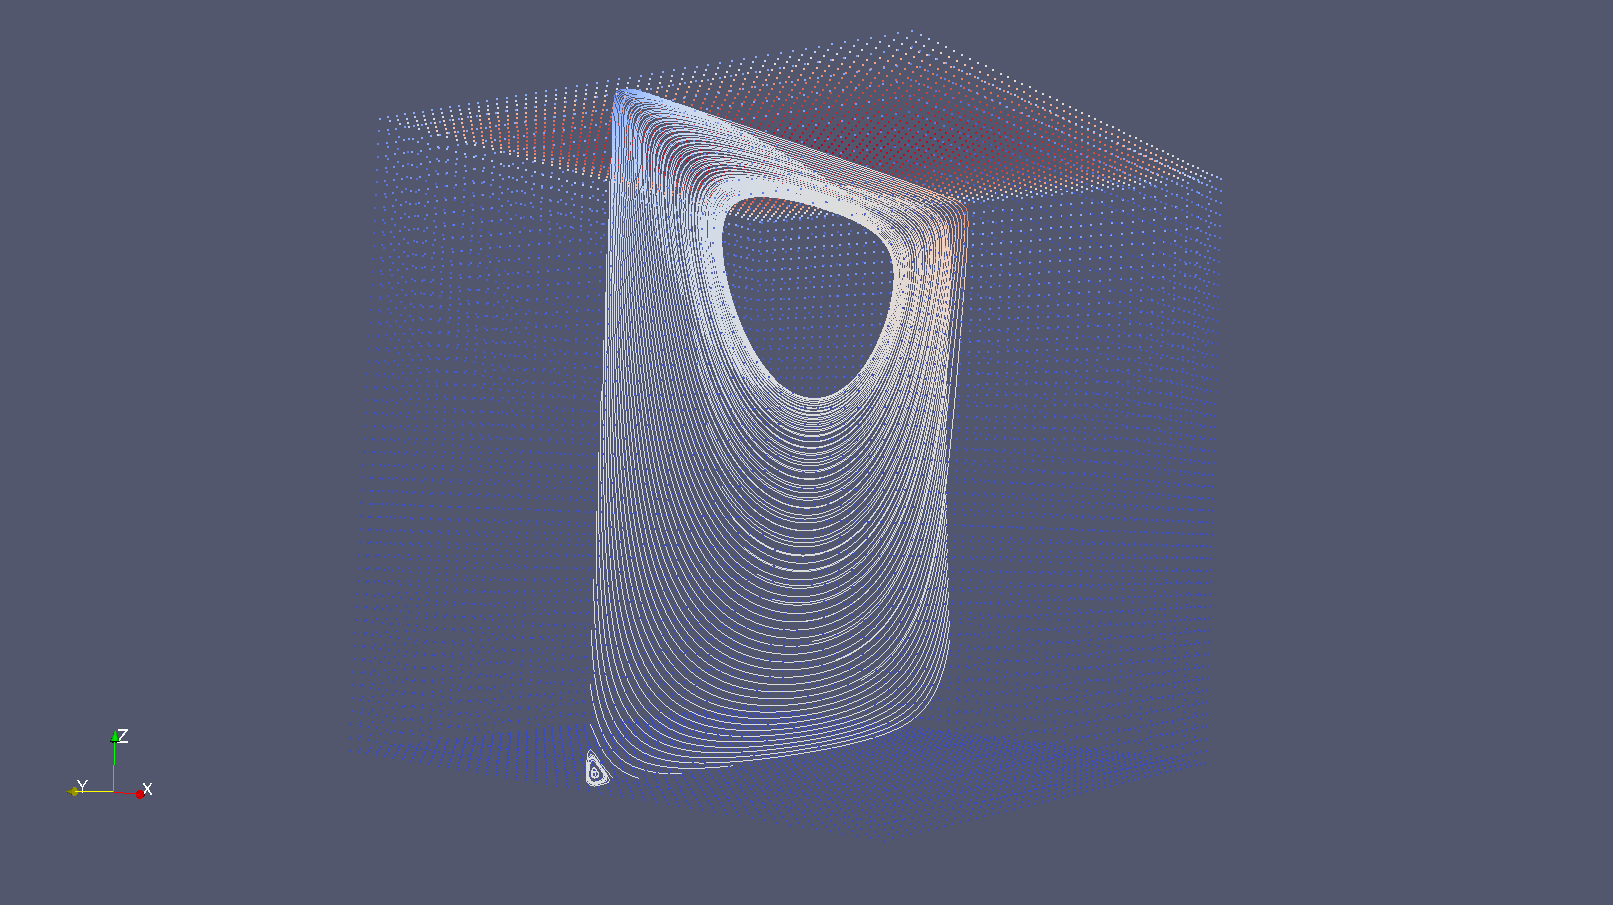
\includegraphics[width=0.7\textwidth]{img/fig10.png}
  \caption{Visualization of the lid-driven cavity simulation with D3Q19 model.}
\end{figure}